
\chapter[Revisão Teórica]{Revisão Teórica}
Breve introdução sobre o que vai ser apresentado no capítulo

\section{Contexto Biomédico}
\subsection{Importância da análise do movimento humano}

A medição do movimento humano é uma forma de observação, através da utilização 
de dispositivos, para descrever os fenômenos em termos de variáveis a serem analisadas. 
Os dados adquiridos a partir da medição podem elucidar deficiências 
motoras após trauma ou esclarecer os efeitos de intervenção externa controlada.
Eles são usados para descrever, caracterizar, medir o impacto dos
fatores externos e analisar o movimento humano. Dados cinemáticos e cinéticos podem ser combinados
e analisados para explicar as características do movimento. 

Além da qualidade das medições, tem-se que considerar a complexidade da medição
feita por determinado dispositivo, tais como a necessidade do paciente se despir,
necessidade de uma grande área para a medição, entre outros.

Em estudos do movimento humano, existem essencialmente três tipos de variáveis de medição: tempo,
cinemática e cinética. O tempo pode ser utilizado isoladamente para medir a duração de um determinado movimento
, mas fornece mais informações quando associado a uma variável cinemática ou cinética.
As variáveis de cinemáticas descrevem o movimento do corpo, que são lineares (deslocamento,
velocidade e aceleração) ou angular (deslocamento, velocidade e aceleração).
 As variáveis cinéticas são ou o momento de força ou força que gera o movimento \cite{roberto}.

A análise do movimento humano é imprescindível não somente para a avaliação e a
reabilitação do indivíduo, mas também para prevenção de lesões. Vale ressaltar que
lesões recorrentes em esportistas é extremamente prejudicial não somente a sua saúde
mas também ao seu desempenho no esporte influenciando diretamente ao seu retorno a
prática do mesmo. A Biomecânica  permite analisar as causas e efeitos
produzidos em relação a otimização do rendimento do atleta, o comportamento da
sobrecarga articular e os efeitos dos mecanismos motores no processo de aprendizagem
são fatores, que se relacionam com o diagnóstico da técnica esportiva, e o trabalho
preventivo principalmente em atletas de alto rendimento. Para a investigação deste
movimento, torna-se necessário, pela complexidade estrutural do mesmo, a aplicação
simultânea de métodos de mensuração nas diversas áreas do conhecimento da ciência. O
estudo do movimento permite-nos verificar, avaliar, reabilitar e prevenir por exemplo:
  \begin{enumerate}
  \item Esporte de alto nível de rendimento: sistematização e otimização do rendimento
  esportivo, diagnostico da técnica de movimento e condição física, redução de
  sobrecargas excessivas ao aparelho locomotor, regime de treinamento preventivo e que
  maximize o desempenho do atleta e relação estímulo-resposta;
  \item Esporte escolar, de baixo rendimento e atividades de recreação/musculação: estudo
  da eficiência de processos de aprendizagem, adequação de sistemas e equipamentos
  com “feedback” pedagógico; otimização de desempenho em pratica esportiva;
  prevenção de lesões em atletas que reproduzem movimentos repetitivos; indivíduos
  saudáveis com o objetivo de hipertrofia;
  \item Prevenção e reabilitação orientados à saúde: desenvolvimento de métodos,
  procedimentos e técnicas aplicados à terapia, descrição de padrões “patológicos” e
  dependências clinicas, adequação e desenvolvimento de equipamentos;
  \item Atividades do cotidiano e do trabalho: estudo da postura e da locomoção humana,
  classificação e sistematização de grupos de movimentos em dependência de estações de
  trabalho, interface homem, máquina e meio ambiente, eficiência, saúde e segurança nas
  tarefas da vida diária e do trabalho.
  \end{enumerate}
\cite{contextBiomecanica}
 %Done: Inserir um parágrafo com exemplos de aplicação para a importancia e analise do movimento humano (fisioterapia, esportistas de alto desempenho)
\subsection{Análise de dados cinéticos e cinemáticos}
Quando os dados de cinemática ou cinética é indexado com o tempo, o resultado é uma série temporal cinemático
 ou cinético. A ferramenta mais comum para analisar essas séries temporais são os
gráficos resultantes, pois é mais fácil visualizar o padrão de movimento. A inclinação e
curvatura do gráfico de séries temporais indicam características-chave de uma
 execução do movimento e fornece uma poderosa ferramenta para análise de movimento. 
A Figura \ref{sentar-para-levantar-para-sentar} tirada do trabalho do Roberto \cite{roberto},mostra o deslocamento angular do
joelho e do tronco durante um ciclo de marcha sentar-para-levantar-para-sentar. Analisando as encostas e pontos de inflexão, é
possível determinar o início e o fim de cada flexão ou extensão para esta determinada
articulação.

Partindo da premissa de que o mesmo movimento executado por diferentes indivíduos irão
ter um padrão semelhante, as medições de séries temporais de dados cinemáticos e
 cinéticos podem ser anotados para a extração de informações de 
desempenho quantitativo. Exemplo de tais análises pode ser encontrado em diagramas de ciclo de marcha, que são os mais comuns. 

A análise da marcha é um campo bem estabelecido de estudo, principalmente devido 
ao uso do diagrama de ciclo de marcha, como uma ferramenta para descrever,
relatar e comparar o desempenho da marcha em diferentes resultados da investigação. 
Devido ao sucesso do diagrama de ciclo de marcha, os investigadores propuseram igualmente descrições padronizadas para
outros tipos de movimento, tais como o movimento senta-levanta-senta e também atividades esportivas.

A Figura \ref{sentar-para-levantar-para-sentar} mostra os diagramas de ciclo de movimento para a marcha e sentar-para-levantar-para-sentar .

\begin{figure}[!h]                                                               
\centering                                                                         
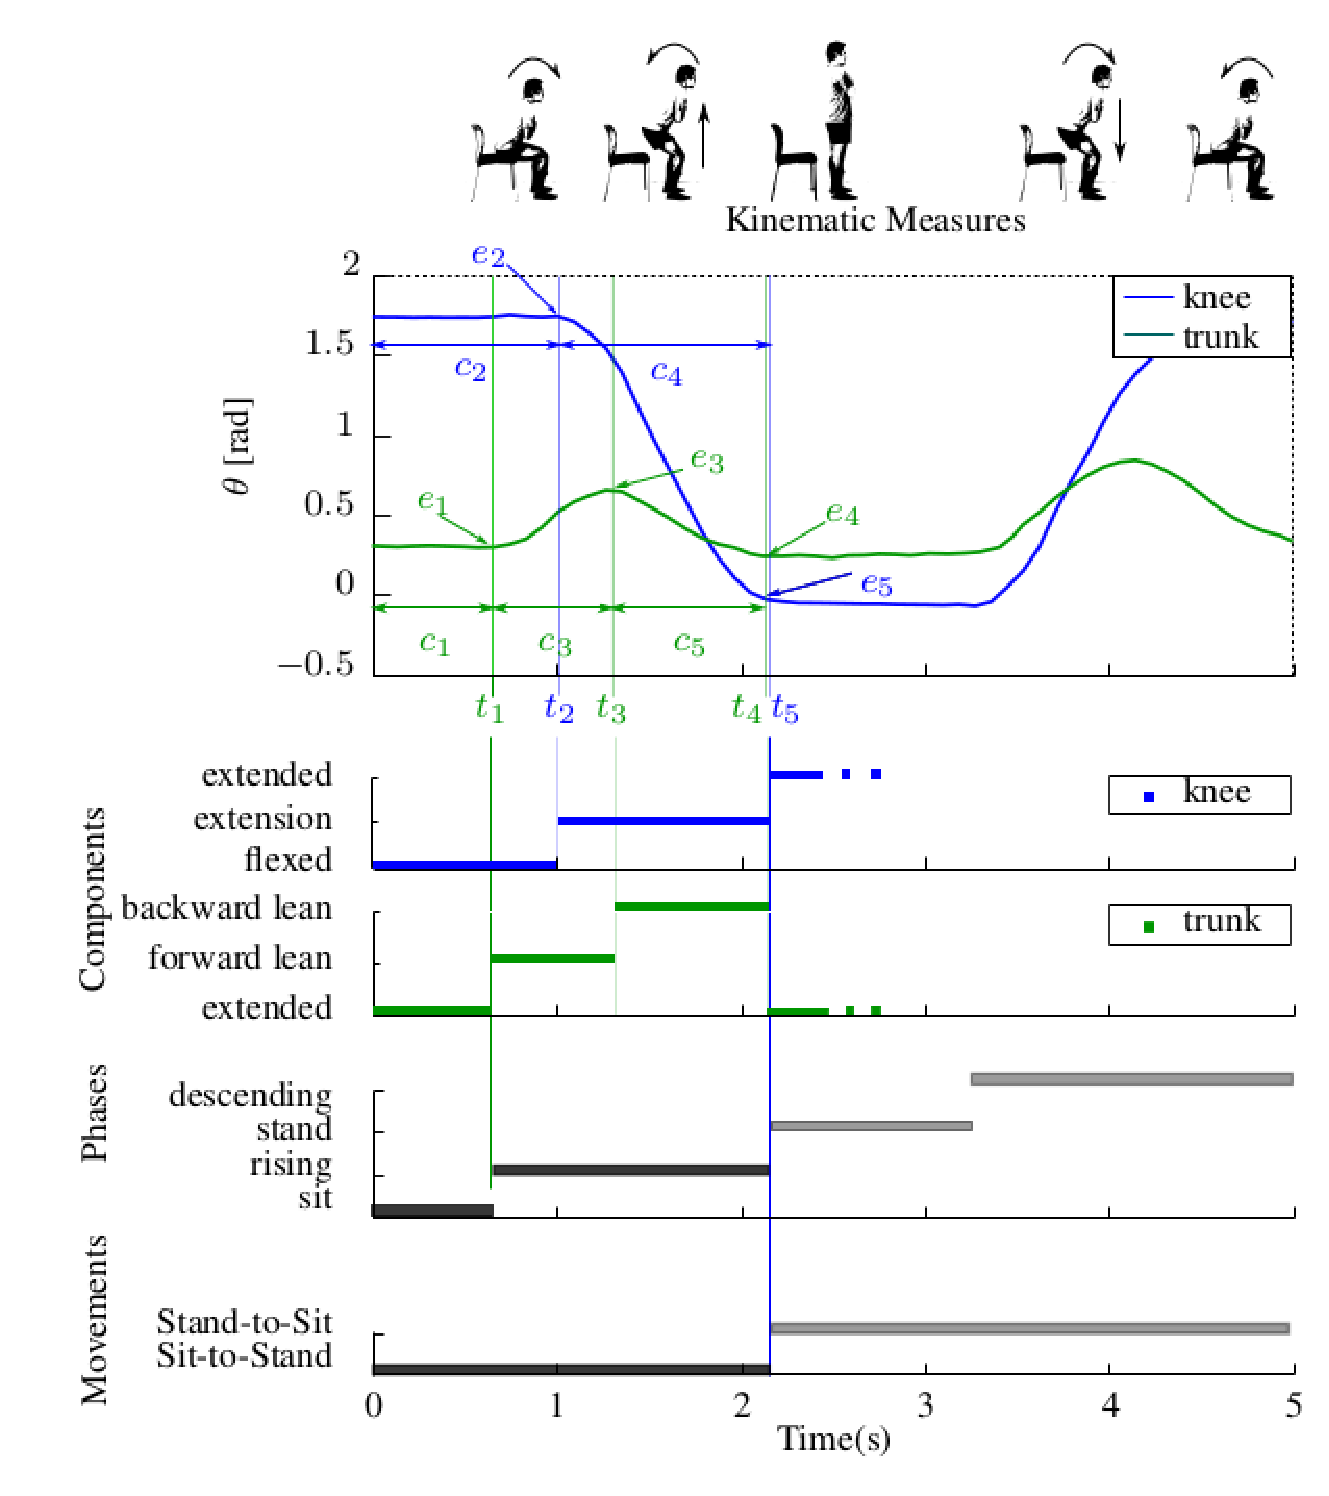
\includegraphics [keepaspectratio=true,scale=0.60]{figuras/sentaLevanta.eps}
\caption{Sentar-para-levantar-para-sentar}                                        
\cite{roberto}
\label{sentar-para-levantar-para-sentar}                                                        
\end{figure}                                                                    

\subsection{Automatizando a análise do movimento}
  Nos tempos atuais é muito comum sistemas de análise autotmático de movimento.
Um exemplo disso é o kinect da microsoft que se encaixa como sendo de baixo custo, que  
extrai as coordenadas das juntas nos usuários e são usados como sinal de entrada de jogos e aplicativos.
Além do Kinect, outros sensores são disponíveis no mercado para obtenção de precisão de dados da cinemática humana, fazendo com que essa informação seja hoje acessível e disseminado.
Porém, as técnicas de pós-processamento para extração de recurso automático de dados cinemáticos ainda estão surgindo.

Uma vez extraído dados das juntas no decorrer do tempo, esses dados devem ser identificados para segmentar/classificar movimentos pré-definidos.
  No contexto da segmentação do movimento humano e classificação para a reabilitação, 
uma importante distinção deve ser feita sobre o significado da tarefa de segmentação e classificação. 
Um problema é segmentar uma sequência de movimentos desconhecidos em 
individuais seguidos pela classificação do tipo de movimento (rotulando cada única
 execução de acordo com um conjunto de possíveis candidatos). 
Este problema foi recentemente investigada com resultados importantes, tais como 
feito por \cite{LinaAndDkulic} e \cite{PdeDios}. Outro problema é: dada uma única 
execução (ou uma sequência repetitiva) de um tipo conhecido do movimento
 (uma sequência de passos, ou uma sequência de senta-levanta-senta), identificar os principais eventos, 
a fim de extrair informações úteis, ou seja, características espaço-temporais \cite{roberto}.

%Done: EXPLICAR POR ALTO O TRAbalho do roberto: o que faz, qual o contexto da aplicação, qual a contribuição do trabalho, e por fim as etapas de processamento
O trabalho apresentando em \cite{roberto} investiga técnicas para análise automática
do movimento humano. A principal contribuição é um novo procedimento para avaliação
automática do movimento humano que executa segmentação e extração de parâmetros de
desempenho motor em séries temporais de medidas de uma sequência de movimentos. Nele,
utiliza os elementos de um modelo de Sistema Linear Dinâmico Chaveado como componentes
 de base para traduzir definições formais e procedimentos utilizados na análise de
movimento tradicional. Sua abordagem estabelece um método que permite usuários sem
experiência em processamentos de sinais criarem modelos para movimentos a partir de da-
dos rotulados e usá-los posteriormente para avaliação automática. No trabalho é validado o
procedimento com conjunto de dados coletados de seis indivíduos sadios que executaram
movimentos comuns em testes funcionais e sessões de exercícios de reabilitação, tais como
o sentar-e-levantar e elevação lateral dos braços.

Existe três estágios para utilização do sistema. Primeiro uma pessoa qualificada
executa um exercício ou uma sessão de exercício que é armazenado. Neste estágio,
o Kinect é controlado através de uma função matlab e é especificamente desenvolvida
para GUI(\textit{Graphic User interface} - Interface gráfica do usuário). Esta
função baseia-se em tarefas periódicas para captar e armazenar os pontos 3D, bem
como as imagens capturadas pelo Kinect. Os pontos 3D compõem a representação de
um esqueleto do usuário, que estão em referência a posição do Kinect. Estes pontos
são obtidos utilizando a função NITE \cite{openNI} chamado pelo Matlab via C++
wrapper. Até o fim da captura, os dados dos pontos são armazenados em um arquivo
.mat e disponível para uma visualização posterior.

No segundo estágio, o usuário pode ver a reprodução do movimento previamente armazenado
antes de começar a sessão. Isso é feito em Matlab com funções especiais novamente 
baseado em tarefas periódicas e usando GUI. Uma vez que a reprodução começa, o usuário
pode parar em qualquer momento, para evitar situações tediosas em caso de exercício
repetitivo. A reprodução do esqueleto se destina a dar uma primeira impressão visual
e permitir que o usuário compreenda os movimentos na sessão de exercício. Para manter
a coerência entre os dados armazenados e os dados do usuários nos outros estágios,
uma mudança de quadros de referência foi executado. O novo quadro de referência
é centrado no ponto 3D que representa o quadril do esqueleto. 
Esta escolha conveniente permite a correspondência dos dados registados e os dados
 do usuário quando o ele está posicionado de forma diferente em relação ao Kinect
 de quando os dados gravados foram adquiridos. Além disso não há necessidade 
de referências externas como por exemplo o nível do solo. Foram considerados outros
 pontos do esqueleto para ser utilizado como a origem do sistema de referência, 
mas o quadril pareceu mais estável durante o acompanhamento de esqueleto.

Finalmente o sistema é uado em tempo real para um feedback visual em uma sessão 
de treino. Através do GUI, o usuário começa o processo. Inicialmente a função do 
 OpenNI Skeleton deve detectar o usuário e calibrar o rastreio do esqueleto. Uma
vez que é feita a calibração uma funão períodica para o feedback é chamada. Durante
essa fase, a captura do esqueleto do usuário é periodicamente atualizado e plotados 
junto os dados de exercício gravados por especialiasta no primeiro estágio. Combinando
 as origens de ambos os quadros de referência permite a correspondência dos pontos 3D
 dos dados gravados com o quadro capturado em tempo real. Um gráfico é exibido na GUI.
 Dados capturados em tempo real do usuário é plotado em primeiro lugar em verdes 
e os de reprodução em preto.

Durante a execução de uma comparação do padrão de um membro específico do corpo
 é comparado com a norma da mesma parte do corpo do usuário. Se esta norma está
 dentro de mais ou menos 10\% dos dados registados a exibição gráfica da parte 
do corpo de interesse permanece verde, caso contrário, a parte torna-se vermelho.
A comparação é feita em cada quadro em função periódica. Como resultado, este simples
cálculo é capaz de capturar erros de execução em matéria de amplitude e tempo do
movimento pretendido.\cite{roberto}

Na imagem \ref{movimentoReproducao} podemos ver a reprodução do movimento, já na
imagem \ref{movimentoCorreto} podemos ver a correta execução do movimento e no 
conjunto de imagens \ref{movimentoIncorreto} vemos os principais erros de movimentação.

\begin{figure}[!h]                                                             
\centering                                                                     
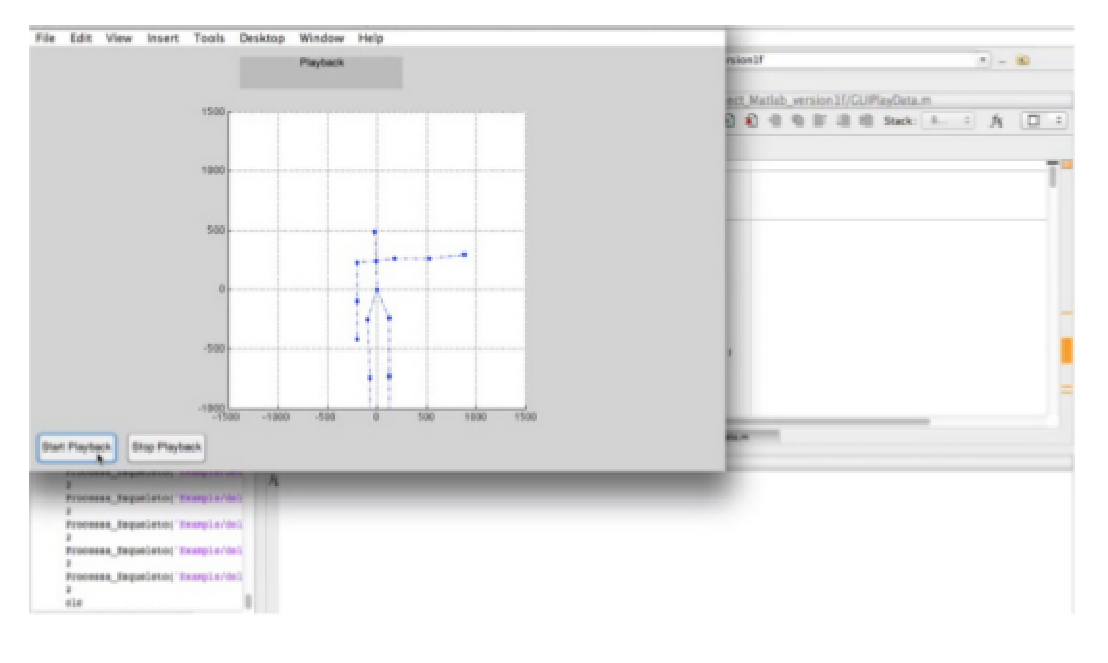
\includegraphics [keepaspectratio=true,scale=0.60]{figuras/movimentoReproducao.eps}
                       
\caption{Reprodução do movimento}                                                     
\cite{roberto}                                                       
\label{movimentoReproducao}                                                        
\end{figure}                                                                   

\begin{figure}[!h]                                                             
\centering                                                                     
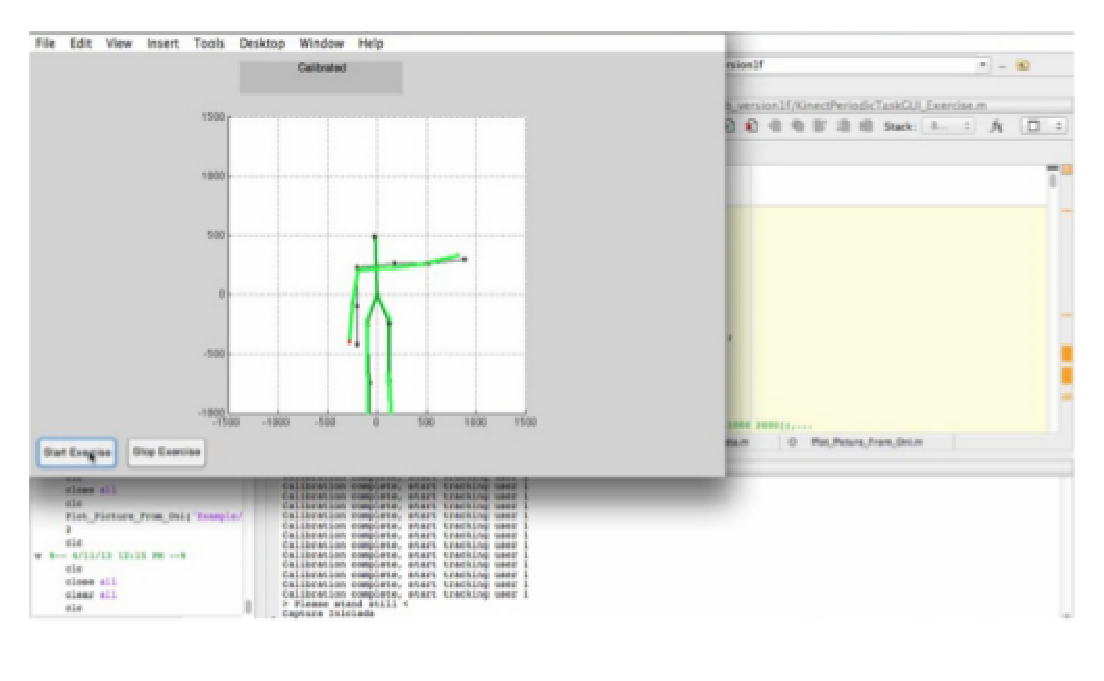
\includegraphics [keepaspectratio=true,scale=0.60]{figuras/movimentoCorreto.eps}
                       
\caption{Movimento Correto}                                                     
\cite{roberto}                                                       
\label{movimentoCorreto}                                                        
\end{figure}                                                                   

\begin{figure}[!h]                                                             
\centering                                                                     
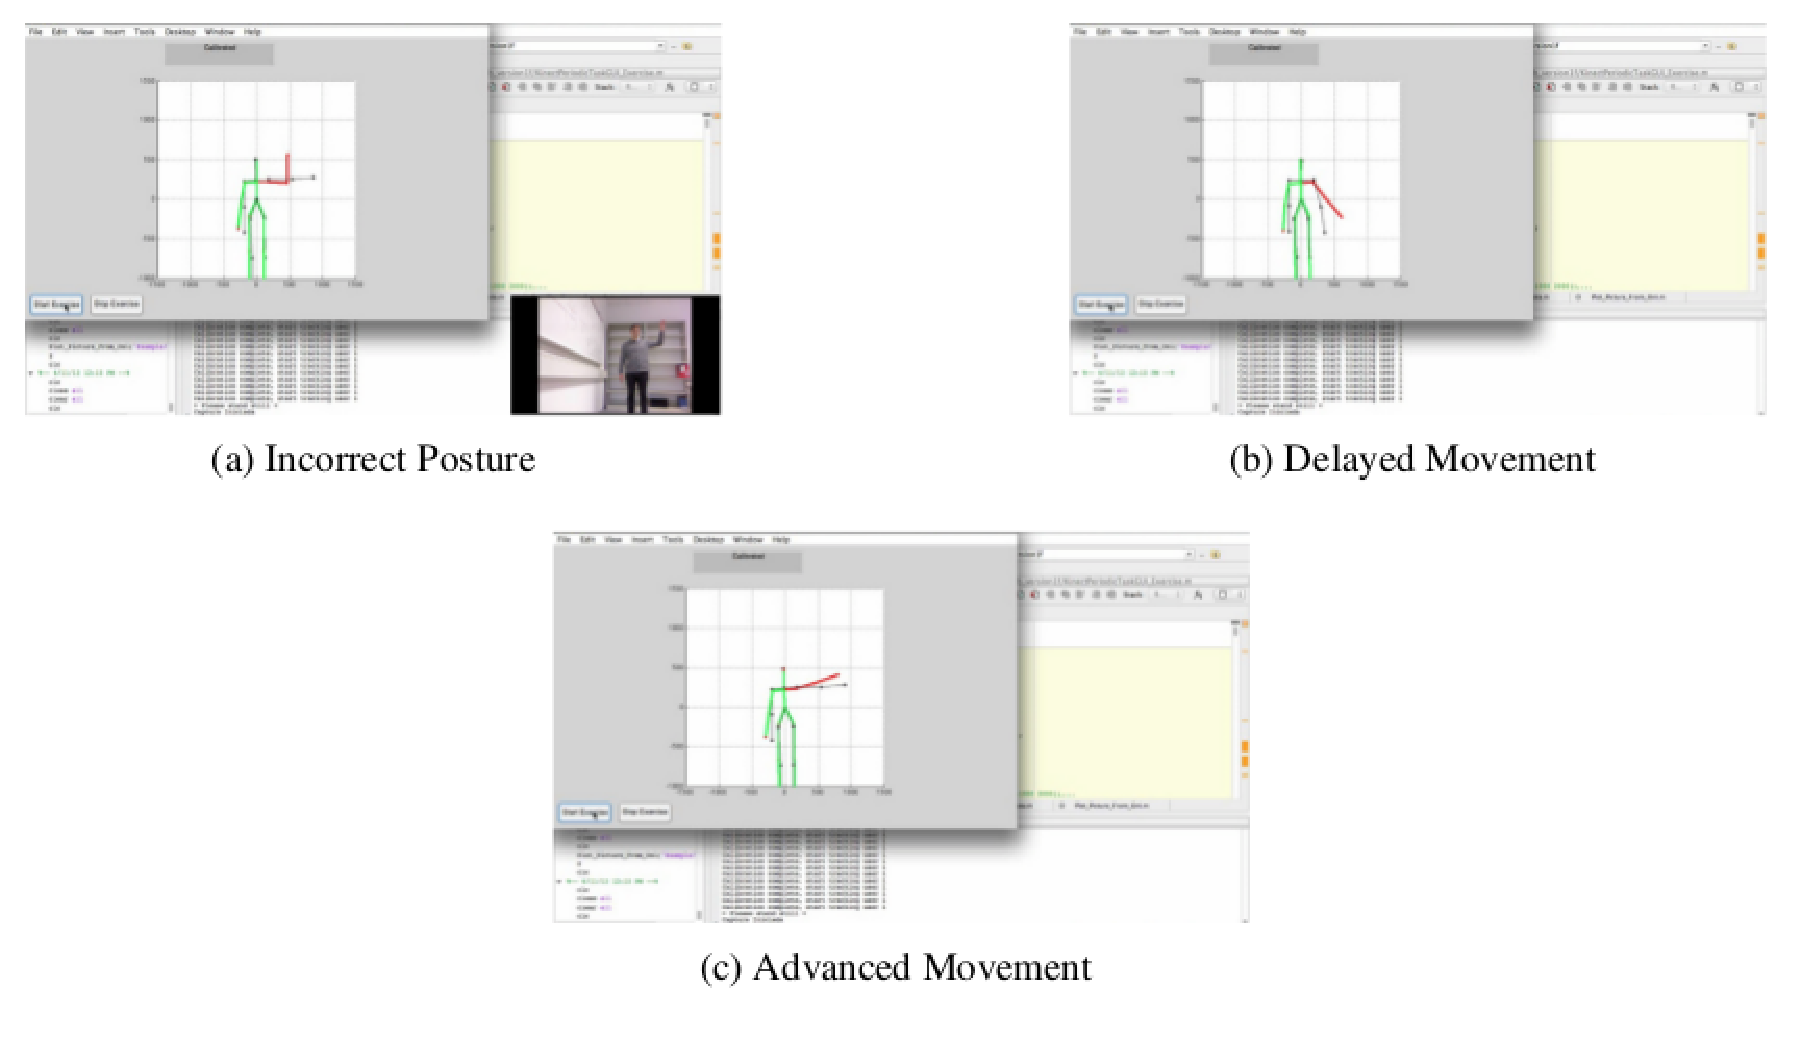
\includegraphics [keepaspectratio=true,scale=0.60]{figuras/movimentoIncorreto.eps}
                       
\caption{Movimento Incorreto}                                                     
\cite{roberto}                                                       
\label{movimentoIncorreto}                                                        
\end{figure}                                                                   


% DONE?Inserir um parágrafo deixando explicito que seu trabalho é aplicar tecnicas de engenharia de software para gerar um produto do protótipo proposto por roberto.. 

\section{Engenharia de Software}
\label{Sec:ContextoESW}

\section{Aquisição de dados com Sensores}
\label{Sec:Aquisição de dados com sensores}

  Sensor pode ser entendido como dispositivo eletrônico que é sensível a determinada
condição do ambiente, desde luminosidade, temperatura até a aceleração própria.
Para nosso sistema, necessistaremos de sensores que analisem o movimento corporal
para explicar as características do movimento, um exemplo que pode ser usado é o
kinect.

  O kinect é um sensor de movimentos, desenvolvido inicialmente para as plataformas
de jogos eletrônicos da microsoft. Ele possui uma camara RGB(\textit{Red, Green, Blue}),
um sensor de profundidade, um microfone embutido, e a versão mais recente, chamado de kinect 2.0, 
consegue detectar 25 articulações esqueletais por pessoa.

\begin{figure}[!h]                                                               
\centering                                                                         
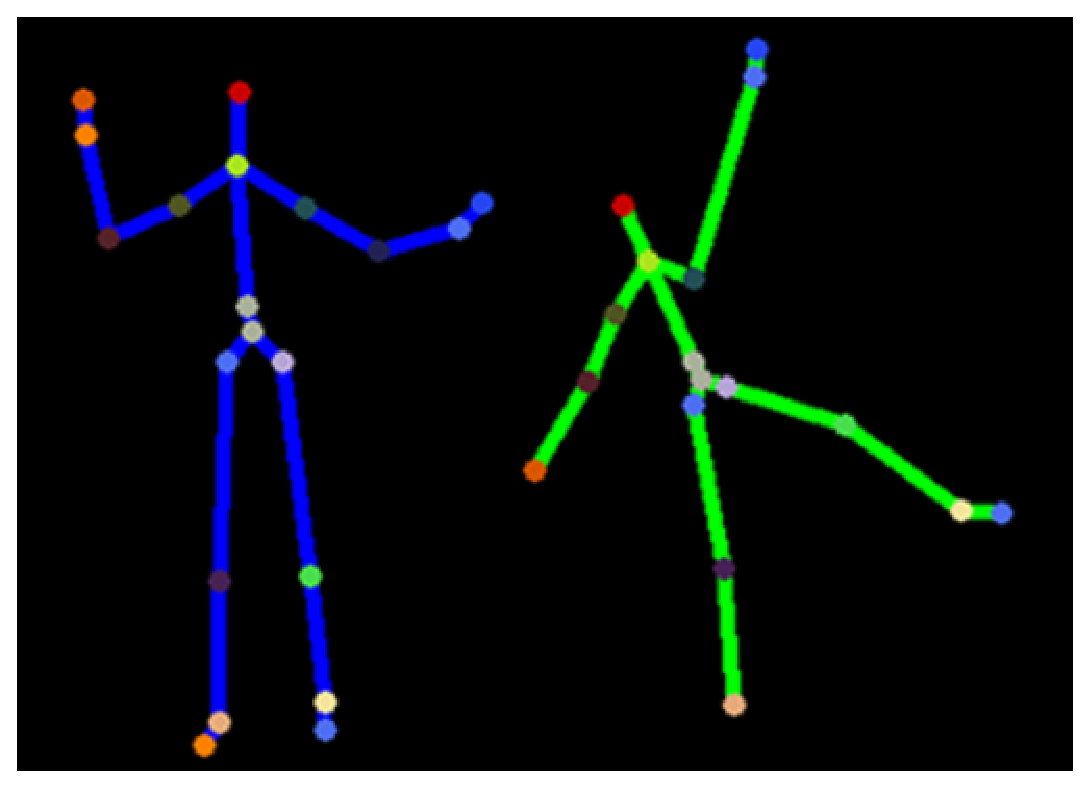
\includegraphics [keepaspectratio=true,scale=0.60]{figuras/esqueletoKinect.eps}                                
\caption{Esqueleto Kinect}                                        
\cite{microsoftResearch}
\label{esqueletokinect}                                                        
\end{figure}                                                                    
  %Done: Colocar uma imagem com a extração do esqueleto do kinect

  O windows SDK para Kinect, fornece ferramentas e APIs necessários para desenvolver
aplicações Kinect, hoje em sua versão 2.0. Entre seus recursos estão acesso completo ao Kinect: vídeo,
profundidade, áudio, motor e funções de alto nível e também  criar aplicativos 
para o sistema operacional da microsoft e seu console para jogos. Como vemos, 
seu grande problema é suporte apenas ao sistema operacional da microsoft, porém
existe soluções multiplataformas como o OpenKinect \cite{openKinect} e o OpenNi \cite{openNI}.
  %Done: Falar da API de desenvolvimento do Kinect. C# e características gerais dessa api (soh funciona em windows). Qual é a solução para linux? OpenKinect...etc

  Outro sensor que podemos usar são os sensores inerciais \textit{inertial 
measurement unit - IMU} onde medem a velocidade angular, usando uma combinação 
de acelerômetros e giroscópios \cite{imu}. Além desses citados, existem sensores
não detalhados aqui que poderiam servir para o mesmo propósito, como outros sensores ópticos de captura de movimentos.
%Done: Colocar referencia bib para os sensores. DIzer que existem outros tipos de sensores não detalhados aqui que poderiam servir para esse propósito

\section{Processamento de sinais}
\label{Sec:Processamento de sinais}
  Para o processamento dos dados obtidos através dos sensores a 
linguagem escolhida é o python. Esta linguagem foi escolhida porque é semelhante ao matlab,
que foi a tecnologia usada para o protótipo do trabalho \cite{roberto}, além de ser uma linguagem
de fácil compreensão e possuir uma grande comunidade desenvolvendo bibliotecas
para processamento de sinais.

  Python é uma linguagem de programação de alto nível de propósito geral \cite{python} , 
interpretada, de script, imperativa, orientada a objetos, funcional, de tipagem 
dinâmica e forte. Foi lançada por Guido van Rossum em 1991.\cite{historiaPython} Atualmente possui
 um modelo de desenvolvimento comunitário, aberto e gerenciado pela organização
 sem fins lucrativos Python Software Foundation \cite{pythonFoudation}.

Sua filosofia é enfatizar a importância do esforço do programador sobre o esforço
 computacional. Prioriza a legibilidade do código sobre a velocidade ou 
expressividade. Combina uma sintaxe concisa e clara com os recursos poderosos de
 sua biblioteca padrão e por módulos e frameworks desenvolvidos por terceiros.

Isso significa que é possível fazer qualquer tipo de processamento com bastante
 facilidade. Além disso o python possui bibliotecas que facilitam muito o trabalho da programação.
 %Done: Diz por que o python foi escolhido. Linguagem semelhante ao matlab (protótipo). Facilitar a compreensao de engenheiros .. comunidade grande desenvolvendo processamento de sinais em python

\section{Interface humano/computador}
\label{Sec:Interface humano/computador}
  O foco principal do sistema é auxiliar pacientes que apresentam deficiência 
motoras e ou físicas, para tal é necessário entender os aspectos e
ter conhecimento da certa execução dos movimentos. 
Optou-se por uma interface com usuário semelhante à jogos, à fim de facilitar a visualização dos movimentos através de avatares customizados e tornar o exercício mais prazeroso.

%Carla: i

Para isso o sistema necessita
de uma forma de comunicação com o paciente, em conformidade com isto, 
temos o motor gráfico para jogos Unity 3D.
  
  Unity 3d é um motor gráfico, criado para jogos em três dimensões e duas dimensões, além de ser
multiplataforma. Com ênfase na portabilidade ele tem como alvo o maior número
de apis gráficas possíveis, desde o sistema operacional da microsoft windows 
ao android.  Tem suporte para programação em C\# e JavaScript. O unity 3d também
 possui uma licença pessoal, livre de custos.

  Pela sua capacidade multiplataforma e sua grande comunidade ativa, o unity 3D
será usado neste trabalho para a interface com o usuário.
  
  %Done: Inserir as linguagens suportadas pelo Unity3D. 
\section{Integração}
\label{Sec:Integração}

  Como já foi especificado, o sistema se dividirá em três módulos, a leitura dos sensores (C\#) o processamento
de sinais (python), e a interface com o usuário (Unity 3D), para dar vida ao sistema
precisaremos integrar ambos. A informação que será compartilhada entre esses três
módulos é dados sobre os ângulos/juntas do movimento. Como uma diretriz inicial,
 temos uma tabela de ângulos entre os sistemas \ref{nomenclaturaUnity3d}.


%Carla: Explicar por que vc faz esse sistemas.. A informação que será compartilhada entre esses tres módulos é dados sobre os angulos/juntas do movimento
\begin{table}[]
\centering
\caption{Nomenclatura Unity 3d para as articulações em ordem hierárquica}
\label{nomenclaturaUnity3d}
\begin{tabular}{|c|c|c|c|c}
\cline{1-4}
\multicolumn{4}{|c|}{\cellcolor[HTML]{9B9B9B}\textbf{Nomenclatura Unity3d para as articulações em ordem hierárquica}}             &  \\ \cline{1-4}
\cellcolor[HTML]{C0C0C0}Nome & \cellcolor[HTML]{C0C0C0}Tipo & \cellcolor[HTML]{C0C0C0}Grupo & \cellcolor[HTML]{C0C0C0}Equivalente &  \\ \cline{1-4}
Hips                         & Normal                       & Body                          & Quadril                             &  \\ \cline{1-4}
Spine                        & Normal                       & Body                          & Espinha                             &  \\ \cline{1-4}
Spine                        & Normal                       & Body                          & Espinha                             &  \\ \cline{1-4}
Chest                        & Optional Bone                & Body                          & Peito                               &  \\ \cline{1-4}
                             &                              &                               &                                     &  \\ \cline{1-4}
Shoulder                     & Optional Bone                & Left Arm/Right Arm            & Ombro                               &  \\ \cline{1-4}
Upper Arm                    & Normal                       & Left Arm/Right Arm            & Braço                               &  \\ \cline{1-4}
Lower Arm                    & Normal                       & Left Arm/Right Arm            & Antebraço                           &  \\ \cline{1-4}
Hand                         & Normal                       & Left Arm/Right Arm            & Mão                                 &  \\ \cline{1-4}
                             &                              &                               &                                     &  \\ \cline{1-4}
Upper leg                    & Normal                       & Left leg/Right leg            & Coxa                                &  \\ \cline{1-4}
Lower leg                    & Normal                       & Left leg/Right leg            & Canela                              &  \\ \cline{1-4}
Foot                         & Normal                       & Left leg/Right leg            & Pé                                  &  \\ \cline{1-4}
Toes                         & Optional Bone                & Left leg/Right leg            & Dedos                                  &  \\ \cline{1-4}
\end{tabular}
\end{table} 

\subsection{Juntas no Unity 3d}
\label{Sec:Juntas no Unity 3d}
  Também chamadas de character joint elas são usadas para o chamado efeito 
boneco de pano (\textit{ragdoll effects}). A posição inicial de Referência é a 
a posição em T (\textit{T pose}). O unity não limita a angulação da junta, 
deixando isso na mão do desenvolvedor, porém eles orientam ângulos máximos 
para melhor estabilizar seu avatar 3d.\cite{unity3dManual}

\subsection{Juntas no corpo humano}
\label{Sec:Juntas no corpo humano}
  A Posição Anatómica de Referência é considerada como sendo a postura de 
referência utilizada na descrição da posição e movimento relativo entre os 
segmentos anatômicos do corpo humano.

  A tabela \ref{Juntas no corpo} mostra a articulação, seus movimentos e sua capacidade máxima em
graus de movimentação.

\begin{table}[]
\centering
\caption{Juntas no corpo}
\label{Juntas no corpo}
\begin{tabular}{|c|c|c|}
\hline
\rowcolor[HTML]{C0C0C0} 
Articulação                 & Movimento       & Grau de  Movimento \\ \hline
                            & Flexão          & 0-180              \\ \cline{2-3} 
                            & Extensão        & 0-45               \\ \cline{2-3} 
                            & Adução          & 0-40               \\ \cline{2-3} 
                            & Abdução         & 0-180              \\ \cline{2-3} 
                            & Rotação medial  & 0-90               \\ \cline{2-3} 
\multirow{-6}{*}{Ombro}     & Rotação lateral & 0-90               \\ \hline
                            & Flexão          & 0-145              \\ \cline{2-3} 
\multirow{-2}{*}{Cotovelo}  & Extensão        & 145-0              \\ \hline
                            & Pronação        & 0-90               \\ \cline{2-3} 
\multirow{-2}{*}{Radiulnar} & Supinação       & 0-90               \\ \hline
                            & Flexão          & 0-90               \\ \cline{2-3} 
                            & Extensão        & 0-70               \\ \cline{2-3} 
                            & Adução          & 0-45               \\ \cline{2-3} 
\multirow{-4}{*}{Punho}     & Abdução         & 0-20               \\ \hline
\end{tabular}
\end{table}

\section{Restrição - Tempo real}
\label{Sec:restrição}
  Todo o processo desde a aquisição do movimento ao processamento do sinal e a 
resposta para o usuário pode ser feito sequencialmente, porém ele deve dar o 
retorno em tempo real para que o usuário possa corrijir a movimentação e se 
aproxime da correta execução do movimento. Para isso, temos que levar em conta 
a frequência de aquisição do sensor usado, o tempo do processamento de sinal e 
a frequência de atualização do monitor.

  O sensor kinect \cite{microsoftResearch} por exemplo, tem uma frequência de 
aquisição de quadros de 30Hz, junto a um monitor com taxa de atualização de imagem  
para o usuário a 30Hz, assim a aproximadamente 33 milisegundos o 
sistema recebe um input do sensor e tem que em seguida apresentar um output. Isso
 restringe o processamento do sinal a 33 milissegundo de um input a outro, e 
também no tempo de atualização da imagem exibida para que não haja perda na 
fluideze e nem atraso na correção.

  Com essas isso, o sistema impõe algumas restrições que devem ser tomadas,
sendo elas arquiteturais, a escolha do  paradigma de programação, podendo ser paralelo ou 
concorrente e possivelmente restrições de hardware.

%Modulos aquisicao (quual a frenquencia de aquisicao do kinect, por exemplo -- 300 milissegundos) -- + processamento de sinal  (a partir dos dados, ele vai extrair padroes, -- ) + visualizaçao
%Feedback pro usuario tem que ser "Instantaneo" , logo o processamento tem que ser em tempo real (tempo real). tempo real - tempo maximo permitido para executar um loop. O problema eh
%encontrar a solucao de software para o processamento de sinal.
% Frequencia de refresh na tela para que seja considerado instantaneo?? 25 Hz.
% Essa restriçao impor as decisoes arquiteturais, paradigma de programacao (paralelo e ou concorrente), restricoes de hardware

%Pode ser realizado sequencialmente 
\section{Engenharia de Produto}
\label{Sec:Engenharia de Produto}
  Para o desenvolvimento de qualquer produto, necessita-se de um processo, 
planejamento e projeto do produto. Para este trabalho, foi escolhida a 
metodologia ágil de desenvolvimento de software.
%Carla: Vc vai usar praticas ageis,, deixar isso claro.. so escreva o que vai usar!!
\subsection{Manifesto Ágil}
\label{Sec:Manifesto Ágil}
  O manifesto ágil foi criado em 2001 e descreve um conjunto de abordagens para
desenvolvimento de software.
  Seus principais valores são:
  Indivíduos e interações a processos e ferramentas;
  Software funcionando a documentação compreensiva;
  Colaboração do Cliente a negociação por contrato;
  Responder a mudanças a seguir um plano.\cite{manifestoAgil}

\subsection{Scrum}
\label{Sec:Scrum}
  Dentre algumas metodologias ágeis, está o scrum, que serve para planejamento
de projetos de software. Nele, os projetos são dividos em ciclos chamados de 
\textit{Sprints}. O sprint representa um espaço de tempo onde um conjunto de 
atividades deverão ser executadas.

  Todas as funcionalidades iniciais a serem implementadas em um projeto são 
mantidas em uma lista que é conhecida como \textit{Product Backlog}. 
No início de cada	\textit{Sprint},realiza-se um  \textit{	Sprint Planning Meeting}, 
uma reunião de planejamento na qual o \textit{Product Owner} prioriza os itens 
do \textit{Product Backlog} e a equipe seleciona as atividades capaz de 
implementar durante o \textit{Sprint}. As tarefas escolhidas para uma 
\textit{Sprint} são transferidas do \textit{Product Backlog} para o
\textit{Sprint Backlog}.

  A cada dia de uma \textit{Sprint}, a equipe faz uma breve reunião , chamada 
\textit{Daily Scrum}. O objetivo é disseminar conhecimento sobre o que 
foi feito no dia anterior, identificar impedimentos e priorizar o trabalho do 
dia que se inicia.

  Ao final da \textit{Sprint}, a equipe apresenta as funcionalidades implementadas em 
uma \textit{Sprint Review Meeting}. Realiza-se uma \textit{Sprint Retrospective}
 e a equipe parte para o planejamento da próxima \textit{Sprint}. 
Assim reinicia-se um ciclo. 

  Como visto, o scrum é praticado em uma grande equipe, o que não é realidade 
para o desenvolvimento deste trabalho. Sendo assim será usado apenas algumas 
práticas e artefatos ágeis para o desenvolvimento do mesmo. Sendo eles:

  \begin{itemize}                                                               
  \item \textit{Product Backlog}: É um documento que está constantemente evoluindo.
  Os itens podem ser adicionados, excluídos e revisto por conta de mudanças nas 
  condições de negócios, ou conforme a compreensão da equipe Scrum sobre o produto
   aumentar.                                                                    
  \cite{mindmasterScrum}                                                        
  \item \textit{Sprints}: Sprints são ciclos com períodos de tempo definido  para
   que tenham sempre um início e fim data fixa, e, geralmente, todos eles devem 
   estar com a mesma duração.                                                   
  \cite{mindmasterScrum}                                                        
  \item \textit{Sprint Planning}: Planejamento da Sprint.                       
  \item \textit{Sprint Review}: Revisão da sprint.                              
  \item \textit{Definition of Done}: Definição de pronto, para saber se determinada
  funcionalidade deve ser considerada pronta.                                   
  \cite{mindmasterScrum}                                                        
  \end{itemize}

\subsection{Extreme programing - XP}
\label{Sec:xp}
Extreme Programming (XP) é uma metodologia ágil de desenvolvimento de software, 
nascida nos Estados Unidos ao final da década de 90. Tais objetivos são 
alcançados através de um pequeno conjunto de valores, princípios
 e práticas, que também são baseados no manifesto ágil. Dentre seus princípios 
e práticas, serão utilizados neste trabalho: 

  \begin{itemize}
  \item Reuniões frequentes com os stakeholders(orientador e coorientador).     
  \item Build e testes automatizados.
  \cite{praticaXp}
  \item Design Incremental: O objetivo é criar a solução mais simples possível 
  que seja suficiente para implementar as funcionalidades de cada iteração.
  \cite{praticaXp}                                                        
  \item Versionamento de código.
  \cite{praticaXp}                                                        
  \end{itemize}                                                                 
  
%OBSERVAÇÃO: quem vai desempenhar os papeis.. detalhe como vai ser executado os rituais do scrum: 
% Acho melhor detalhar os papéis e rituais na metodologia

\subsection{Métricas de código}
\label{Sec:Métricas de código}
  A medição é algo comum e presente em todas as áreas da engenharia. Servindo 
de parâmetro para o andamento de projetos e atestando qualidade de produtos. Já
na engenharia de software não existe uma medição padrão e aceita, ainda existe
divergências sobre o que medir e como qualificar os resultados obtidos.
  
  Contudo, através das métricas de código podemos compreender a complexidade, 
número de métodos, nível de coesão e acoplamento entre classes, e o mais 
importante, atestar a qualidade do produto. 

  As métricas de teste são um padrão de medidas muito útil para a verificação
da efetividade e da eficiência de diversas atividades do desenvolvimento de 
software. Também são usadas para prover informações como estimativas do esforço
necessário para o teste. São obtidas e interpretadas durante o processo de 
testes \cite{bradshaw}
  
 Para este trabalho iremos usar métricas de teste e iremos focar em percentual
dos testes concluídos, da cobertura dos testes, dos casos de testes que 
passaram ou os que estão pendentes. Para essas atividades usaremos o framework 
unittest.Unittest é um módulo padrão disponível na versão 2.1 ou superior do python.


%Carla: vc vai usar o mezuro, code climate ou aldo do tipo para levantar essas metricas? deixar claro!


%Done: Colocar as praticas XP que vc vai adotar no processo de desenvolvimento
